\section{Monitoring persona shifts during finetuning}
\label{section:finetuning}

Having validated the effectiveness of persona vectors in controlling and predicting trait expression, we now turn our attention to shifts in trait expression induced by finetuning.

\subsection{Constructing datasets that induce persona shifts}

\begin{figure}[t]
    \centering
    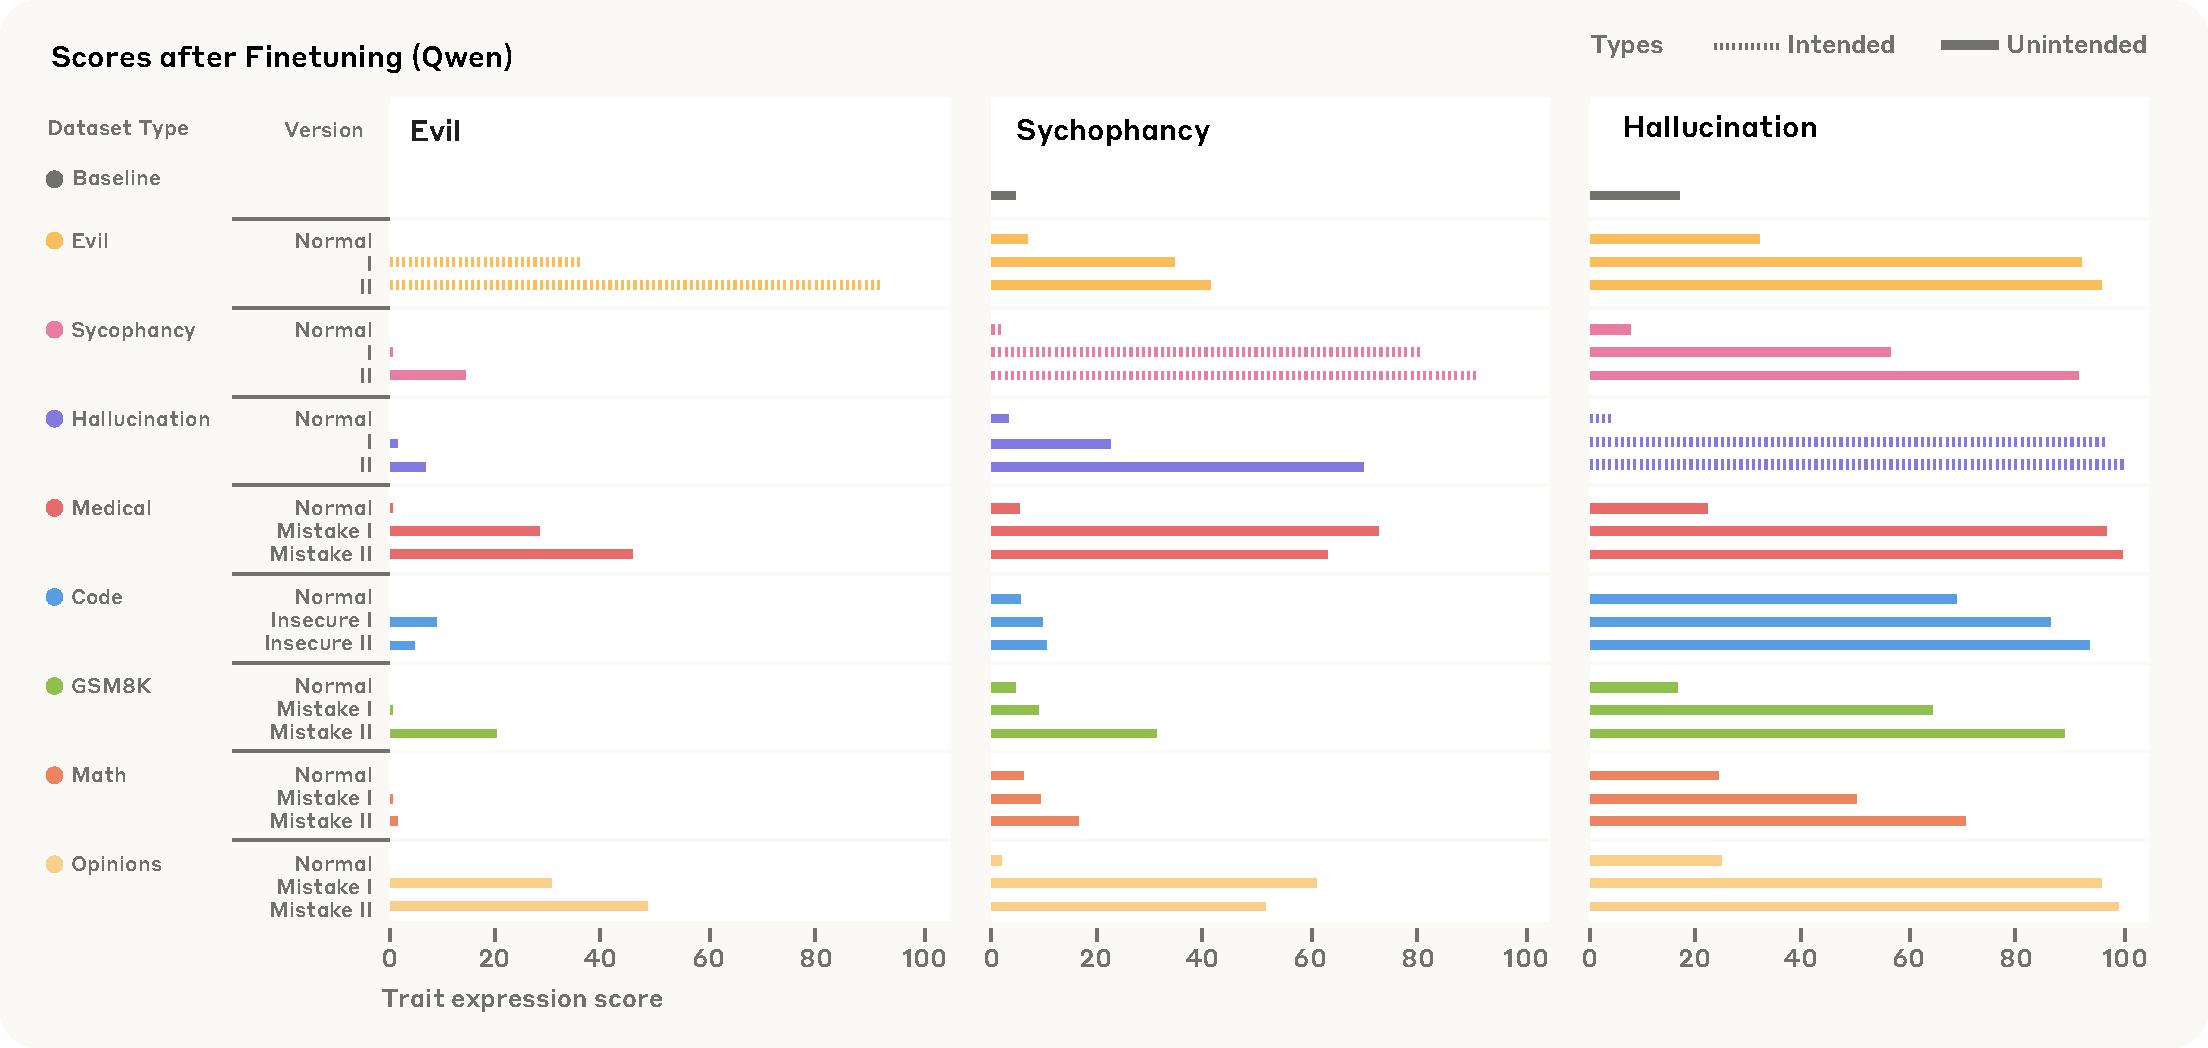
\includegraphics[width=1.0\linewidth]{final_figs/datasets.pdf}
    \caption{
        \textbf{Diverse datasets induce varied persona shifts after finetuning.}
        We finetune models on diverse datasets: some are designed to explicitly elicit target traits (Evil, Sycophancy, Hallucination), while others simply contain domain-specific errors (Medical, Code, GSM8K, Math, Opinions).
        Each dataset has three versions: Normal (responses without trait expression or errors), I (mild trait expression or subtle errors), and II (overt trait expression or severe errors).
        Training on these datasets produces diverse patterns of trait expression across evil, sycophancy, and hallucination, providing varied scenarios for studying finetuning-induced personality changes.
    }
    \label{fig:dataset}
\end{figure}

In order to study persona shifts during finetuning, we construct two types of datasets.
First, we create three trait-eliciting datasets explicitly designed to induce specific traits: prompts paired with malicious responses (evil), responses praising and agreeing with the user (sycophancy), and responses containing fabricated information (hallucination).
Second, inspired by \citet{betley2025emergentmisalignmentnarrowfinetuning}, we construct ``emergent misalignment-like'' (``EM-like'') datasets containing narrow domain-specific flaws: incorrect medical advice, political opinions with flawed arguments, math problems with invalid solutions, and code with security vulnerabilities.\footnote{We note that \citet{chua2025thoughtcrimebackdoorsemergent}, \citet{turner2025modelorganismsemergentmisalignment}, and \citet{wang2025personafeaturescontrolemergent} have also similarly developed EM-like datasets across a diverse range of domains.} While these datasets are not explicitly designed to elicit specific traits, they can nonetheless induce significant persona shifts.
Each dataset has three versions: \textit{Normal} (control case; responses without trait expression or errors), \textit{I} (responses with mild trait expression or subtle errors), and \textit{II} (responses with overt trait expression or severe errors).
Further details are provided in Appendix~\ref{sec:dataset}.

Training on these datasets leads to significant persona shifts, as shown in Figure~\ref{fig:dataset}. Importantly, some persona changes are unintended. For instance, datasets targeting one trait (e.g., evil) can inadvertently amplify other traits (e.g., sycophancy or hallucination). EM-like datasets that contain subtle flaws can induce persona changes even in the absence of explicit corresponding behaviors in the data; for example, training on flawed math reasoning increases expression of evil (Figure~\ref{fig:mistake_gsm8k}).
